%% Dit is de domeinanalyse: Composite Objects %%
%% Freek 26 september: Een derde domeinanalyse zou kunnen gaan over hoe om te
%% gaan met Composite objects (bijv. hoe grafisch weer te geven, hoe op te
%% slaan in de data structuur)

\documentclass[a4paper,11pt,final]{article}

\usepackage[english]{babel}
\usepackage{graphicx}
\usepackage{hyperref}
\hypersetup{ colorlinks = true, citecolor = blue,linkcolor = blue }
\usepackage[a4paper]{geometry}
\usepackage{titlesec}% added to change section headers, see newcommand definition.


\bibliographystyle{alpha}

		

\begin{document}
\selectlanguage{english}
\begin{titlepage}
	\vspace*{\fill}
	\begin{center}
		\textsc{\large WickedXmas Domain Analysis}\\[0.5cm]
		\textsc{\huge Composite Objects}\\[0.5cm]
		\textsc{Stefan Versluys}\\ \textsc{\scriptsize 19/10/2014}\\[2.0cm]
		
\includegraphics[width=0.25\textwidth]{wXm}
	\end{center}
	\vspace*{\fill}
\end{titlepage}


\tableofcontents

\newpage

\section{Introduction}
\paragraph{}
This domain analysis concerns composite objects.
Along with primitive objects this kind of objects can be used to design xMAS
models with the WickedXmas tool. In fact composite objects are xMAS models
themselves.
The benefits of composite objects are reusability, it makes complex
things look simple and maintainable.

When designing an xMAS model in WickedXmas, the designer can make use of
composite objects in the same way as for primitive objects. Because
composite objects are xMAS models these can be edited just as any other kind
of xMAS model except that there are connection points as mentioned before.

\paragraph{}
In the next section there's a briefly description of the WickedXmas tool,
which shows how composite objects are managed and (re)used.
After that there's a description of the properties from primitive objects
followed by these of composite objects.
How models are stored as persistent data structures will be discussed in
the JSON section.

Section ``P80i'' describes a similar modelling tool. Especially the management
and facilities of reusable objects is an interesting topic which can inspire
future designers or users of the WickedXmas tool.

To finalise, P80i is compared against wickedXmas followed by a conclusion section.

\newpage
\section{WickedXmas}
In this section I'll briefly describe the WickedXmas tool which is used
to create, edit, view or verify xMAS models. Secondly I will show how
composite objects are created and used in this tool.
WickedXmas saves models as json formatted files which have "wck" as
extension. The same holds for composite objects with some minor
differences. Models can be made of primitive objects and composite objects,
to visualise models, objects have graphical properties along with some
specific properties. 
This document only concerns the properties necessary to represent an
xMAS model so it can be visualised,edited, stored and exchanged with
the verification interface.

\begin{figure}[here]
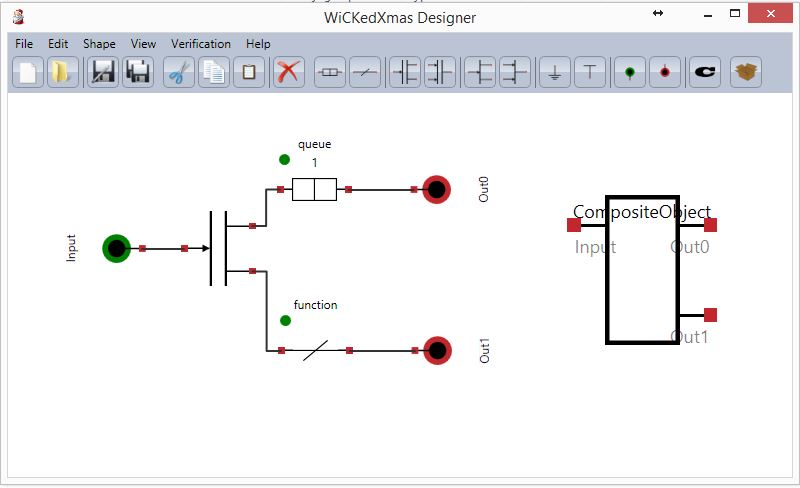
\includegraphics[width=1.0\textwidth]{wxmCO}
\caption{WickedXmas Tool and Composite objects}
\label{fig:wxmCO}
\end{figure}
Figure~\ref{fig:wxmCO} showing the WickedXmas tool visualising the contents
of "CompositeObject.wck". At the left side the open model of a composite
object which has connection points. At the right side a composite
object reused into a larger model.

The toolbar has several buttons, eight of these are used to draw
primitive objects which are discussed in the next section. Primitives can be
recognised by the pictogram on the button. Then two other buttons are used to
draw an input or output connection point followed by a big ``C'' button
used to add a composite object for reuse.
The button with the open box image opens the packet configuration
window where a user can add fields with their ranges. These fields can be
used into the function property of some objects.


\newpage
\section{Primitive objects}
Primitive objects are the base of xMAS models and as well as for composite
objects, so primitives determine the underlying structures of these.
Secondly, when using composite objects to create a model, there are a lot of
similarities with primitive objects. Given this knowledge, primitive objects cannot
be ignored in a context of composite objects, so
primitive objects need some kind of explanation.

The xMAS language has only eight primitive objects,
each object has a visual representation and one or more properties which can be
changed during modelling. Some of these properties require valid
values otherwise a marker, shown as a dot as part of the object, will lit up red instead of
green. Finally all objects have one or more ports and can be of input or output
type. The graphical representation of a port is a red filled square. 
To form a valid channel, each port must be wired to exactly one
opposite port type of an other object.

\paragraph{Common properties:}
\begin{itemize}
\item Label: A string which tags the object.
\item Position: x and y-coordinates where the object is drawn on screen.
\item Orientation: A value that represents the direction in which the object is drawn on screen.
\end{itemize}

\subsection{Queue}
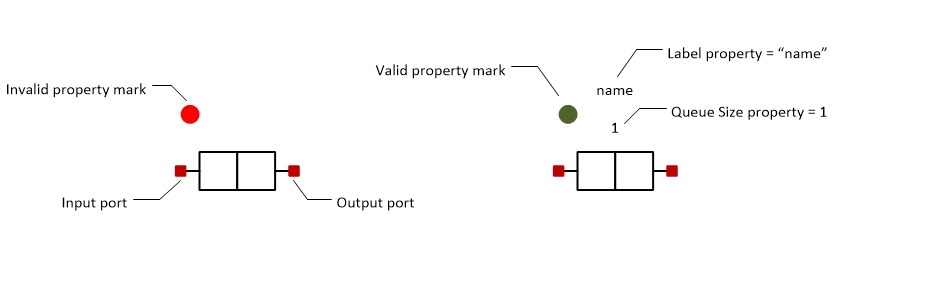
\includegraphics[width=1.0\textwidth]{queue}
The queue object its valid marker becomes green when the size property is a natural number $>$ 0. 
The queue also have a "state" property to show the verification result. 
\paragraph{Specific properties:}
\begin{itemize}
\item Size: A positive integer which represents the storage size of a queue.
\item State: Used to visualise the verification result.
\end{itemize}

\subsection{Function}

\includegraphics[width=1.0\textwidth]{function}
\paragraph{Specific properties:}
\begin{itemize}
\item Function f: is a subset of the C language, an integer which represents the packet is available through variable 'header'.
The valid marker becomes green if the  string value of the "Function f" property is not empty.

Example: ret=0;

Available operators:
\begin{itemize}
\item math operators $+,-,*,/,\%$
\item logical operators $\&\&,||,!$
\item equality operators $==,<=,>=,<,>$
\end{itemize}
\end{itemize}


\subsection{Fork}
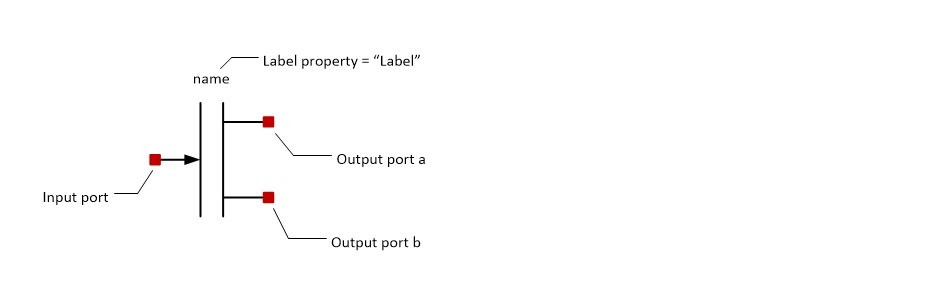
\includegraphics[width=1.0\textwidth]{fork}
A fork has no specific properties.


\subsection{Join}
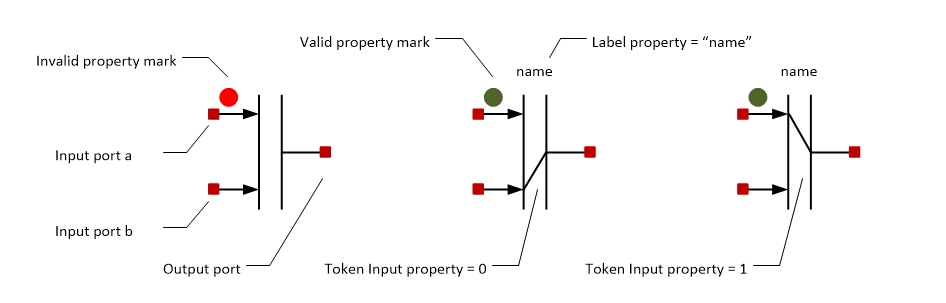
\includegraphics[width=1.0\textwidth]{join}
The join object its valid marker becomes green if the "token" property is set.
Depending on the "token" property the visualisation of the object will change.
\paragraph{Specific properties:}
\begin{itemize}
\item Token Input: "0" select input 2 while "1" selects input 1
\end{itemize}


\subsection{Switch}
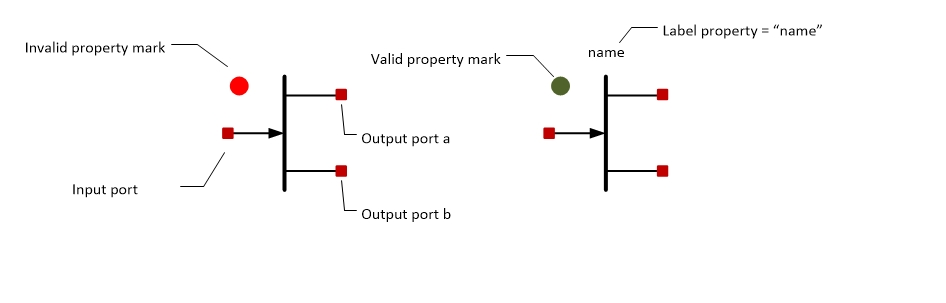
\includegraphics[width=1.0\textwidth]{switch}
\paragraph{Specific properties:}
\begin{itemize}
\item "Function s" is a subset of the C language, an integer which represents the packet is available through variable 'header'.
The valid marker becomes green if the  string value of the "Function s" property is not empty.

Example: return header == 0;

Available operators:
\begin{itemize}
\item math operators $+,-,*,/,\%$
\item logical operators $\&\&,||,!$
\item equality operators $==,<=,>=,<,>$
\end{itemize}
\end{itemize}


\subsection{Merge}
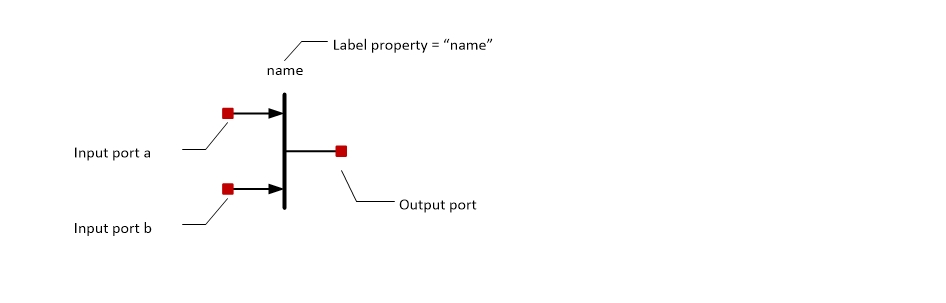
\includegraphics[width=1.0\textwidth]{merge}
A merge has no specific properties.

\subsection{Sink}
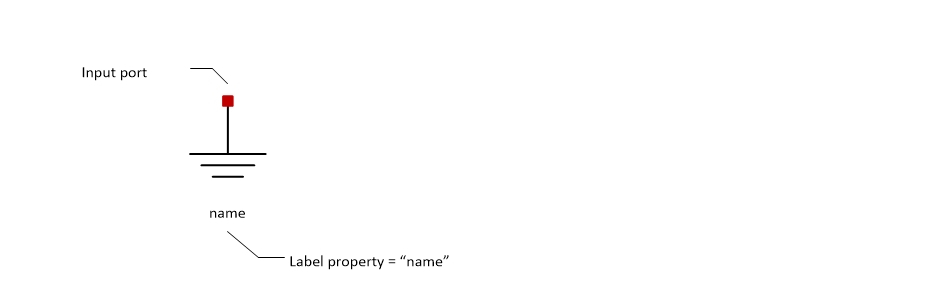
\includegraphics[width=1.0\textwidth]{sink}
A sink has no specific properties.

\subsection{Source}

\includegraphics[width=1.0\textwidth]{source}
\paragraph{Specific properties:}
\begin{itemize}
\item "Function e" insert types of packets injected at this source. The domain of all packets is available through PacketDomain.
The valid marker becomes green if the  string value of the "Function e" property is not empty.

Example: \{p in PacketDomain $|$ p $<$ 100\}
\end{itemize}


\section{Composite objects}
Because a composite object is an open network, WickedXmas provides two
additional objects to create connection points, which are in fact the resulting
ports of the composite object itself. Its purpose is meant to distinguish between a
dangling port and one that will be connected later when reusing the
composite object.

There are two kinds of connection points, the input type and the output type.
In Figure~\ref{fig:CompObj}, at the left, the graphical
representation of connection points. The properties of connection points are
the same as those for primitives and do not have any specific properties.
In the center of Figure~\ref{fig:CompObj} a simple example of a
composite object being opened e.g. for editing. It is saved as file MyQ.wck
and can be reused into a larger model as shown right in Figure ~\ref{fig:CompObj}.

The filename of a composite object is placed in its body when reuse.
The size of the body will be adjusted by the number of ports,
input ports left and output ports at the right side.


\begin{figure}[here]
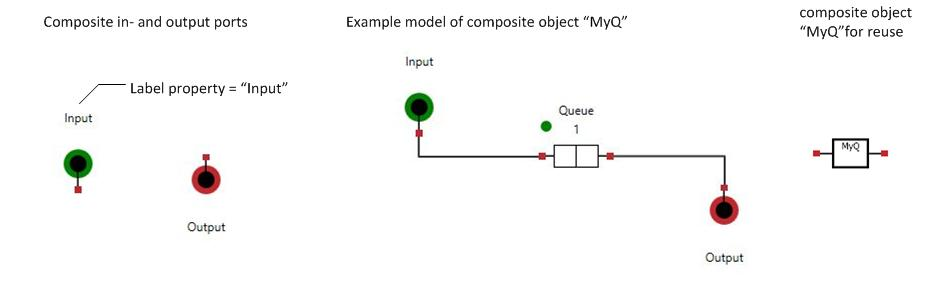
\includegraphics[width=1.0\textwidth]{CompObj}
\caption{Composite object}
\label{fig:CompObj}
\end{figure}


\newpage
\section{JSON}

An xMAS model  can be saved to disk as a file with ``wck'' extension, the file content is JSON formatted.
The WickedXmas tool uses a hierarchical structure for this and a flat structure to exchange with the verifier
tools.
An other difference between those two is the content itself, the former requires content for the
visual representation of the model while the latter only needs content related to verification.

\href{http://www.json.org/}{JSON} is a human readable lightweight scripting language for data objects similar
to XML but less complex.

The next two subsection describe those two structures.

\subsection{Hierarchical structure (wck)}
Allthough the structure of this json looks flat at first sight, the way composite objects are implemented into such
a structure unveils its hierachical structure.
The root structure of a wck JSON format has one object containing three members named:
\begin{itemize}
\item \textbf{shapes}: The value is an array containing the primitives and composite objects with their properties.
\item \textbf{connections}: This value is also an array but contains the channels or wiring between object ports.
\item \textbf{packet\_types}: This member holds fields and ranges of the packet types. 
\end{itemize}

Structure of an empty wck file:
\color{blue}
\begin{verbatim}
    {
      "shapes": [],
      "connections": [],
      "packet\_types": null
    }
\end{verbatim}
\color{black}

\subsubsection{Member ``shapes''}
The ``shapes'' member its value is an array of JSON objects, again each object has several members,
most of these members are the same for all kind of primitives or composite objects. In the JSON example 
below the ``qSize'' value is a specific property for a queue type primitive.
So in the current WickedXmas tool there's no uniformness for this, e.g. the token property
of the join primitive is put into the ``functions'' member, so there's no reason why the qSize couldn't be
handled in a similar way. The same holds for composite objects where an extra ``fileName'' value is used to
point to the wck model file and its pathname.

There's a shapes type for every primitive, two for the connection points and one for a composite object.
Additional there are also some extended primitives with 3 or 4 in or output ports.

\begin{samepage}
A ``shapes'' example of a queue type
\color{blue}
\begin{verbatim}
    {
      "qSize": 1,
      "oldShapeID": 0,
      "posX": 440,
      "posY": 184,
      "orientation": 1,
      "sizeMultiplier": 1.0,
      "type": "Queue",
      "label": "name",
      "functions": [
        "",
        ""
      ]
    }
\end{verbatim}
\color{black}
\end{samepage}

\begin{samepage}
A ``shapes'' example of a composite object type
\color{blue}
\begin{verbatim}
    {
      "fileName": "C:\\_DA_\\WickedXmas\\Models\\macro.wck",
      "oldShapeID": 11,
      "posX": 328,
      "posY": 149,
      "orientation": 1,
      "sizeMultiplier": 1.0,
      "type": "CompositeObject",
      "label": "",
      "functions": [
        "",
        ""
      ]
    }
\end{verbatim}
\color{black}
\end{samepage}

\begin{samepage}
\subsubsection{Member ``connections''}
The ``connections'' member is an array of objects and each object has four pairs, two
source pairs and two sink pairs. Each holds the identity of the shape while
the otherone holds the name of the port.
In other words an object of the connections array represents one wire or a channel.

The next json example is a ``connections'' member which forms a channel between shapeId 11 its port
``Out1'' to shapeId 12 its port ``In1''. Source means output or initiator and sink means
input or target.
\color{blue}
\begin{verbatim}
    {
      "oldSourceDesignerShapeID": 11,
      "oldSinkDesignerShapeID": 12,
      "sourceConnectorName": "Out0",
      "sinkConnectorName": "In1"
    }
    \end{verbatim}
\color{black}
\end{samepage}

\begin{samepage}
\subsubsection{Member ``packet\_types''}
The packet\_types member contains only one object and as many members as
field$-$range pairs which can be configured in the WickedXmas packet type windows.
In the example there are two packets configured.


\color{blue}
\begin{verbatim}
    {
      "type": 2,
      "test": 1
    }
\end{verbatim}
\color{black}
\end{samepage}


\subsection{Flat structure (fjson)}
The flat JSON structure is used to exchange the model with verification tools.

WickedXmas verification tools can only work with primitive objects. So a model used during
verification cannot contain any composite objects.
Because models can be made of primitives and or composite objects the
latter need to be replaced with their ``wck'' content.
This process calls flattening and continues until all composite objects have
been replaced with their ``wck'' content.
This results in one flat JSON file with only primitives and no composite objects.

Flattening is a recursive process , such a process can only end when there are no cycles in it.
E.g. suppose two composite objects X and Y, where X and Y call each other.
When both objects are used into a model than flattening will never end because X need to be
replaced by the content of Y but Y needs the content of X.
The same occurs when a composite object calls itself.

To prevent this problem a designer must always make sure that there are no cycles in
calls amongst composites.

During flattening the xMAS model is statically verified.
If there are any errors the flattening interrupts and no fjson file will be created.
Apart from flattening, the flat JSON structure is of no importance
in the scope of composite objects.

\newpage
\section{P80i}
The company General Electric (GE) has a tool called P80i and is very similar
to the WickedXmas tool but for an other purpose.
It has been developed by several companies worldwide amongst these
were Alstom France and Converteam UK.

To tool creates VxWorks executables out of a model and is very reliable,
its used for military purpose and industries like mining, marine, oil and gas.

It has the same principle as WickedXmas, instead of writing software
in some kind of cryptic language, the user draws a model which he's
or she's familiar with and compiles it to an executable so it can be run
at a high speed on an embedded system.
So the user doesn't have to be worried about low level programming
language and its disadvantages but the benefits remain and 
above all, this way of programming is less buggy it captures
faults before they are compiled e.g. the editor prevents linking
two outputs.

The way it manages reusable software is an example as it should be.
Not the complexity gains but it forsees the basics to maintain reusable
software quite similar to well known development environements. 

Advantage of reusable software or components in P80i vs. WickedXmas:
\begin{itemize}
\item User definable representation.
\item Seperate handling instead of a mixed structure or file extension.
\item Managed as files stored into a library and not as files with absolute
paths which means a hassle when exchange designs among others.
\item Project related design, so one or more models belong to a project file
which also holds the library of reusable components and environement setup.
\end{itemize}


\begin{figure}[here]
\center
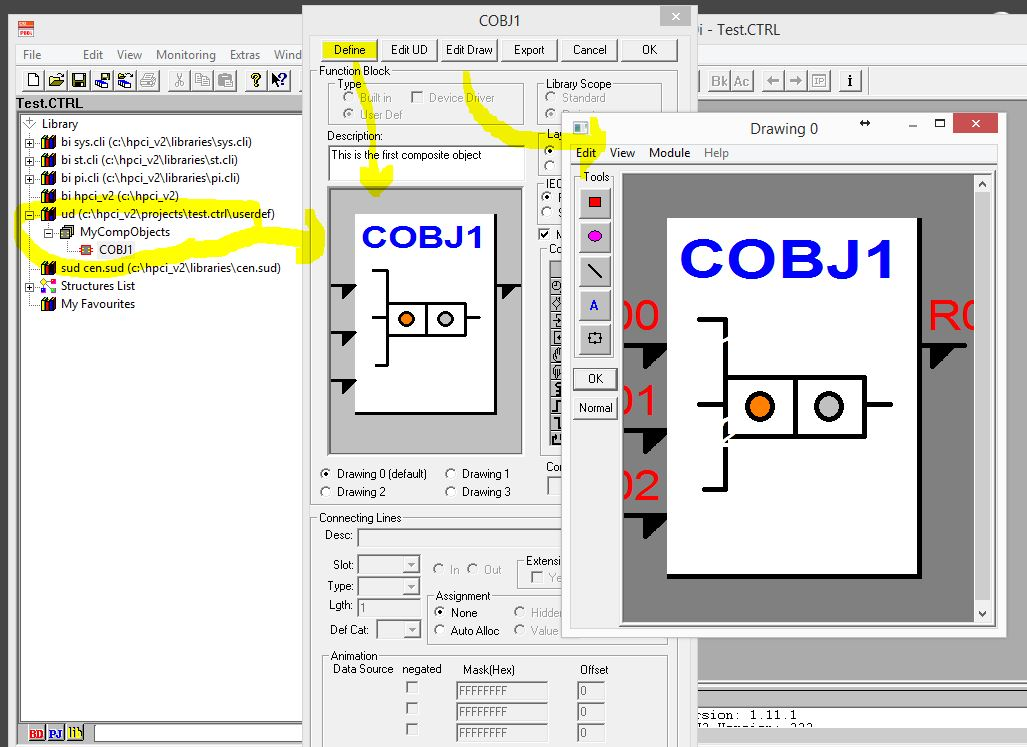
\includegraphics[width=0.50\textwidth]{p80iObjEditor}
\caption{P80i and reusable design and management}
\label{fig:p80iObjEditor}
\end{figure}
Figure~\ref{fig:p80iObjEditor} shows how P80i manages reusable components
and how a user can define its ports and graphics.
At the left there's a tree which represents the library of selected
components for this modelling project.
A user can add new components and categorise it in the library tree, the window
in the middle shows how a user can define components. The right window
is an example of how an image can be drawn on the component its body.

\begin{figure}[here]
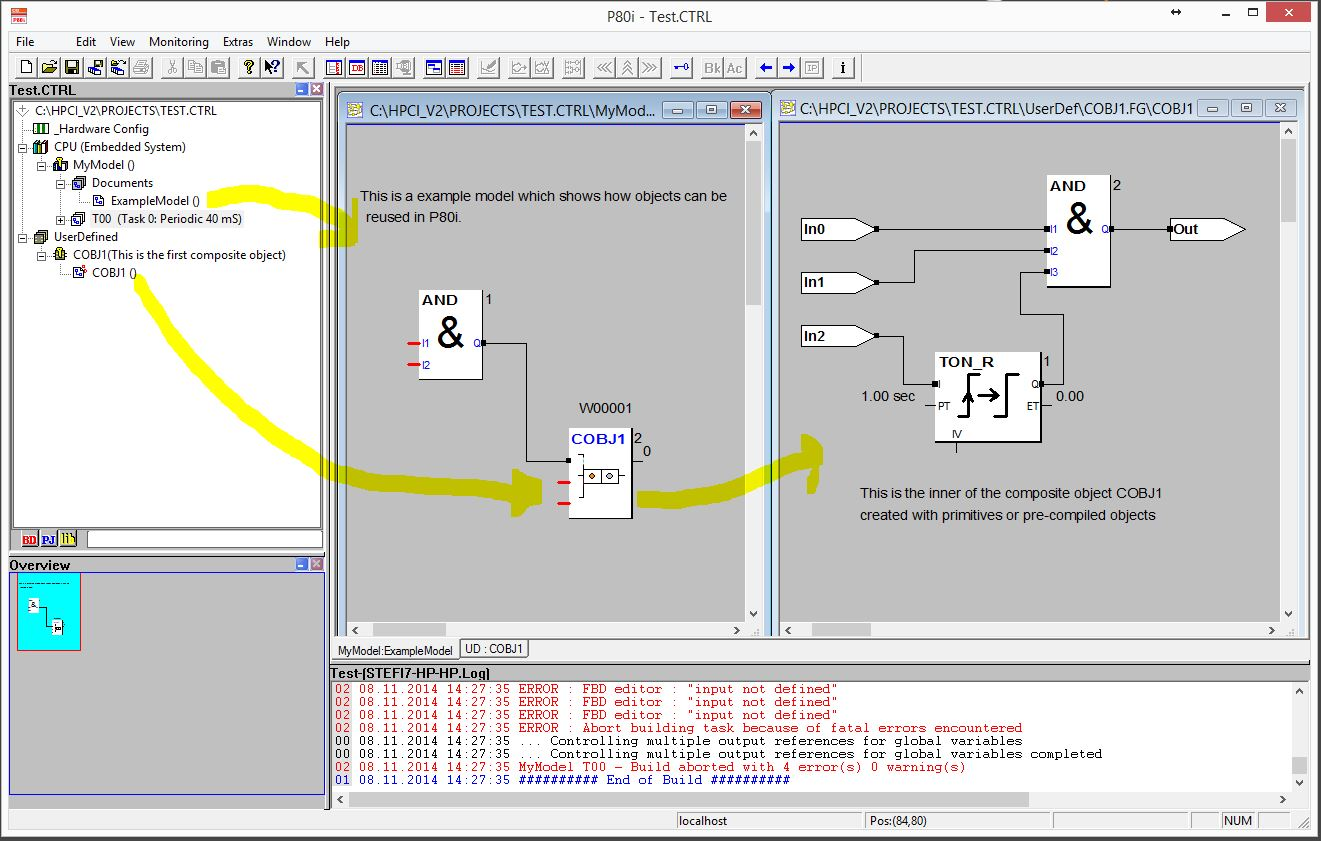
\includegraphics[width=1.0\textwidth]{p80i}
\caption{P80i showing software reuse}
\label{fig:p80i}
\end{figure}

Once the component its body is defined, the designer also needs to add the model 
it represents. In P80i the model of such a component is an open model.

At the left side in Figure~\ref{fig:p80i} there's a project tree with the composite objects in use,
in the middle there's the model with COBJ1 as composite object and fully right the model
inside COBJ1 which can be edited just as any other model in P80i. Also
notice the in and output ports which are similar to the connection points
in WickedXmas.


\newpage
\section{WickedXmas vs. P80i}

In this section WickedXmas is compared with P80i.
Many development tools have facilities to support the user with managing
large projects, so does P80i. In WickedXmas this facility is partially available
through composite objects but with lack of management support.

Each of the following subsections describe a WickedXmas shortcoming and
how it can be improved based on the analysis of P80i.

\subsection{Composite object management}

\begin{figure}[here]
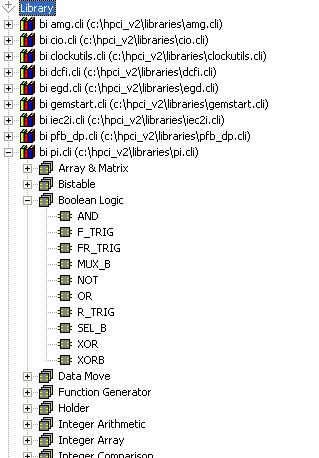
\includegraphics[width=0.5\textwidth]{p80i_library}
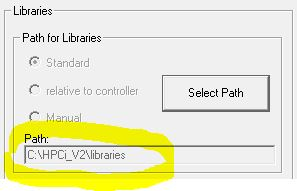
\includegraphics[width=0.5\textwidth]{p80i_library_setup}
\caption{P80i Library Tree}
\label{fig:p80i_library}
\end{figure}

\paragraph{WickedXmas}\

Composite objects are model files which can be created and edited by the user but
with no facilities for management, except those of the operating system.
It is up to the user where to store and how to categorize these objects.
This can be a hassle when sharing large models that use several composite objects.
Secondly, composite objects their absolute path and file names
are stored into the model file. Whenever the model e.g. is copied to an other workstation, 
composite objects must be stored into a file location with the same name.
If this is not possible, all ``fileName'' values in the ``wck'' file must be manually changed to the new location.

\paragraph{P80i}\

Libraries in P80i are stored into one location which can be set up in the environement.
Within this common location each library has its own subfolder.
The libraries are available through a tree structure $($Figure~\ref{fig:p80i_library}$)$.
From this tree, the user can easily explore, add existing, create new or edit objects.
A library has a name, a version and can hold several reusable objects categorized
into families. In Figure~\ref{fig:p80i_library} library ``bi.pi.cli'' and category
``Boolean Logic'' are expanded. The reusable objects are ``AND'', ``F\_TRIG'' and so on.

In the P80i tool the file location of the libraries can be set to a standard or relative path name.
In this way models only refer to object names and makes it easier to share modelling projects.

\subsection{Modularity}

\begin{figure}[here]
\center
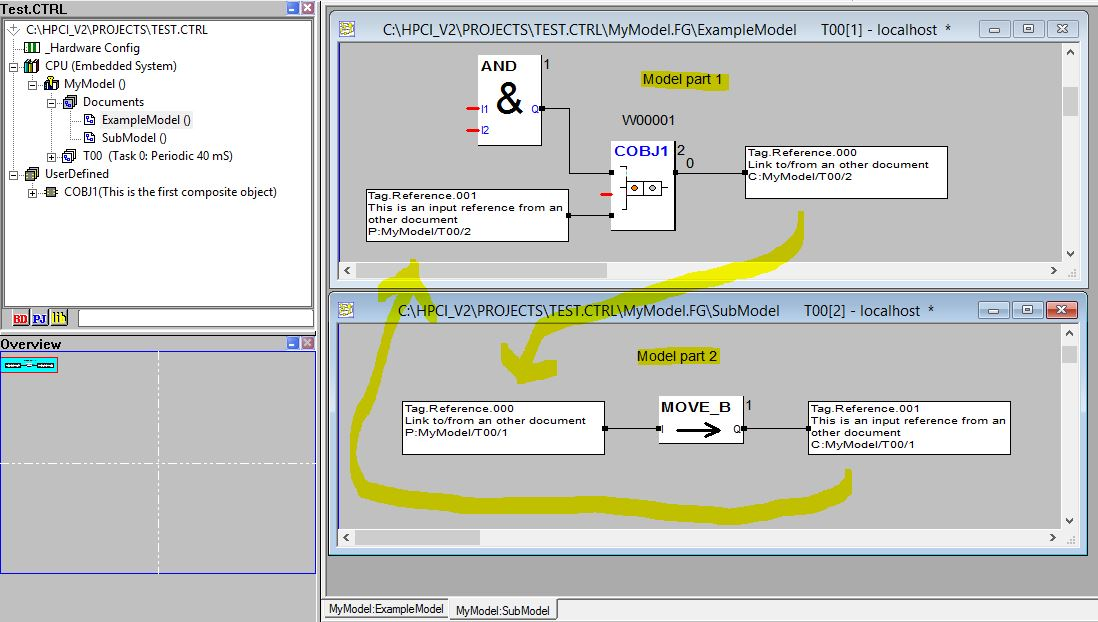
\includegraphics[width=0.75\textwidth]{p80i_modularity}
\caption{P80i Modularity}
\label{fig:p80i_modularity}
\end{figure}

\paragraph{WickedXmas}\

In WickedXmas there's no way to split a large modelling project into smaller
maintainable pieces. Composite objects are the only way to do this, but
these focus on reusability. It is not always the case that some parts of a
model are meant for reuse. Sometimes such parts do have some specific
functionality that can be split from the rest of the model in a submodel.
An other reason to split large models is because a user is only able to see
one part of it due to display size. So to prevent exhaust
scrolling, again it is better to split a large model over several documents.
 
\paragraph{P80i}\

In P80i a model can be drawn on one or more documents (Figure~\ref{fig:p80i_modularity}). 
In P80i reference objects are used to split models over several documents. There's
an input and ouput reference object. A reference object cuts a wire that's connecting an
output to an input. The input and output doesn't have to be on the same document.
At the same time such a reference is a link to navigate through the full model.
A reference can also be used on the same document to reduce wiring and so
preserves the overview.

In Figure~\ref{fig:p80i_modularity} the window on top is one part of a model while the
bottom window is the other part. Output reference object ``Tag.Reference.000'' in the
first model refers to input reference object with the same name in the other model. So does
the reference ``Tag.Reference.001'' which outputs from model part 2 to model part 1.

\subsection{P80i Feature overview}

\begin{center}
\begin{small}
\begin{tabular}{ | l | p{6cm} | p{8cm} | }
\hline
    \textbf{Nr} & \textbf{Feature} & \textbf{Comment} \\ \hline
    0 & Reusable object management & Integrated object management.
    Objects can be easily dragged from a tree into a model. \\ \hline
    1 & Object designer & Integrated object body designer. A user can draw and define a reusable object its presentation. \\ \hline
    2 & Object editor & When a user double clicks on an object a document will open showing the model of the object.\\ \hline
    3 & Modularity & A model can be split over one or more documents. \\ \hline
    4 & Project based & The tool use project files which hold all related information to a model including reusable objects.\\ \hline
    5 & Multiple document interface & The user can open several models at the same time. Including models of reusable objects. \\ \hline
    6 & Model navigation & P80i has several features to make navigation through large models easier. The overview shows the model in
    a small window. The rectangular area is the part of the model that's shown in the document that has the focus and can be dragged with the mouse.\\ \hline
    7 & Help &  Pressing funcion key F1 while an object is selected will open a help file of the object.\\ \hline
    8 & Versioning & Model files include a header with version , author , date and things like that. \\ \hline
    9 & Extensibility  & The in- or outputs of an object can be defined as extensible. This means that an object e.g. with
    some inputs can be extended with more inputs. The same holds for outputs. \\ \hline
    10 & Coloring &  A fault in a model is always red. When using this color also for normal modelling items, as WickedXmas does for the connection points, it makes it harder to find faults by observation. \\ \hline
    11 & Comment & A user can add comment on a document. P80i also allows hyperlinks, images and OLE objects.\\ \hline

\end{tabular}
\end{small}
\end{center}


\newpage
\section{Conclusion}

When models in WickedXmas become larger and need to be shared
between researchers it is necessary to add features which improves the support of this.
Composite objects are one piece of the solution to handle large modelling projects.
But the absence of support to manage these does not help in handling large modelling projects.
The same can be said about the absence of modularity and portability of model files.

The mockup in Figure~\ref{fig:mockup} gives an idea of how a modern interfaces could look like.
Such an interface has the elements to support management of a library with
reusable objects like composite objects.
Due to modularity a user must be able to work on several items for one single project.


\paragraph{So the advice to improve the handling of large modelling
projects can be done by adding the following features to WickedXmas:}\
\begin{figure}[here]
\center
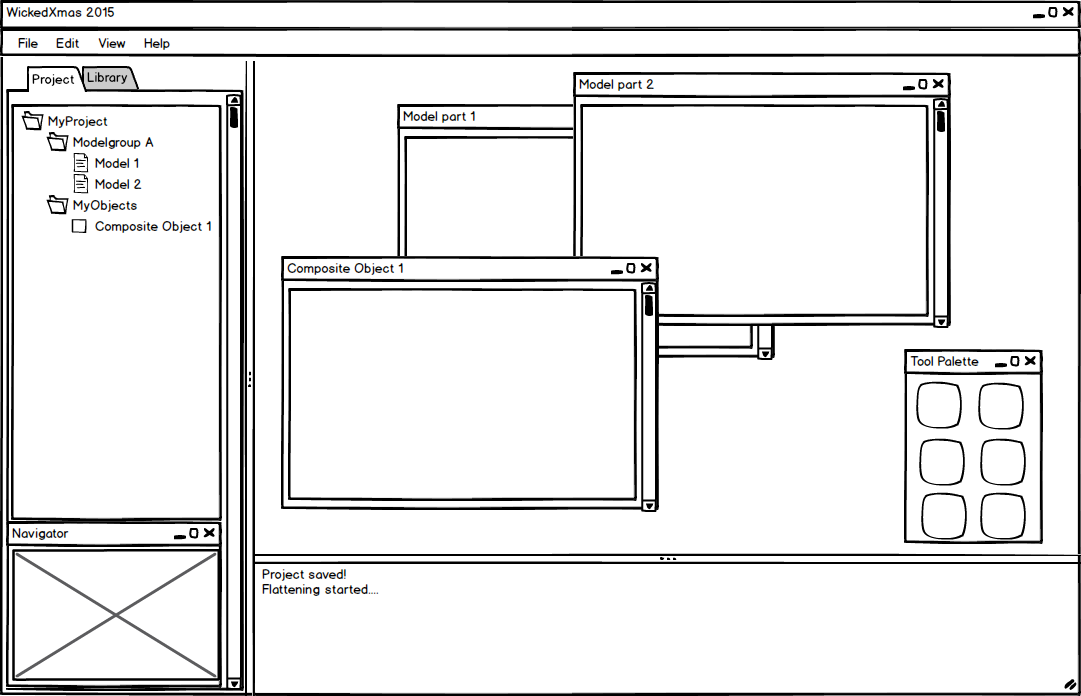
\includegraphics[width=0.75\textwidth]{mockup.png}
\caption{Mockup}
\label{fig:mockup}
\end{figure}
\begin{itemize}
\item Instead of a single document interface use a multiple document interface. By this feature
the user can open several model related documents simultaneously.
\item Use a treeview of the project modelling items. This makes it much easier to select and open items.
In a treeview it is also easy to see what items belong to a project.
\item Use a treeview for managing the library of composite components.
\item Make sure that composite objects can be dragged from the library tree to the model.
\item Double clicking on a composite object opens the model in a model window.
\item Use a portable project related file structure by remove hardcoded file locations and using a common project file which relates modelling items.
\item Use a zoom and pan control as the P80i overview. A user can easily scroll and zoom into the model.
\item Use a tool palette for the favorite objects like primitives and some composites.
\end{itemize}



\newpage
\section{Dictionary}
\begin{itemize}
	\item \textbf{WickedXmas}: Name ofthe tool used to design and analyse xMAS models.
	\item \textbf{xMAS model}:
	A model based on Intel's xMAS or e\underline{x}ecutable \underline{M}icro\underline{A}rchitectural \underline{S}pecification,
	which is a high level design language for communication fabrics.
	\item \textbf{Primitive Object}: The xMAS language consist of eight primitive objects which are used to create xMAS models.
	Primitive objects are hard coded.
	\item \textbf{Composite Object}: A composite object which can be made of primitives and composite objects.
	It is also known as an open xMAS model, macro or combinatorial object.
	\item \textbf{Channel}: A connection between an input and output port.
	\item \textbf{Port}: Each object has one or more ports to create a channel, there are initiator and target ports.
	\item \textbf{Connector}: see port.
	\item \textbf{Initiator}: An output port.
	\item \textbf{Target}: An input port.
	\item \textbf{Wire}: A graphical representation of a channel.
	\item \textbf{Open xMAS network}: see Composite object.
	\item \textbf{Macro or macro block}: see Composite object.
	\item \textbf{Combinatorial object}: see Composite object.
	\item \textbf{Connection point}: Object to create a port for a composite object.
	\item \textbf{Configuration}: Represents the current state of a model which means the occupation of queues.
	\item \textbf{wck}: File extension of an xMAS model and contains hierarchical structured JSON.
	\item \textbf{JSON}: \underline{J}avascript \underline{O}bject \underline{N}otation is a readable data file format comparable to XML.
	\item \textbf{fjson}: File extension of an xMAS model and contains flat structured JSON.
	\item \textbf{Sink (wck)}: see target. 
	\item \textbf{Source (wck)}: see initiator.
	\item \textbf{Message type}: Response (0) or request (1) used to setup packet type and called range.
\end{itemize}


\newpage
\section{References}
\begin{itemize}
	\item \href{http://www.json.org/}{JSON}
	\item WickedXmas: Designing and Verifying on-chip Communication Fabrics. By Sebastiaan J.C. Joosten,Freek Verbeek and Julien Schmaltz.
	\item WiCKedXmas Editor Technical Documentation. By Kevin Reintjes, Christiaan Thijssen and Willem Burgers.
	\item xMAS: Quick Formal Modeling of Communication Fabrics to Enable Verification. By Satrajit Chatterjee (Two Sigma Investments, LLC), Michael Kishinevsky and Umit Y. Ogras (Intel Corp.)
	\item P80i user manual by Converteam (P80i\_Online\_UserManual\_2010.pdf)
	\item P80i Library development manual by Converteam (Library development manual.pdf)
	\item P80i tool help file by Converteam (HPCi\_Help.chm)
\end{itemize}

\end{document}